\documentclass[number]{USG}

% subcaption loaded by USG.cls
\usepackage{listings}
\usepackage[numbers]{NJDnatbib}
\setcitestyle{numbers,square}
\graphicspath{{./figures/}{./wiley/images/}}

% Code listings configuration
\lstdefinelanguage{JavaScript}{
  morekeywords={const,let,var,function,return,if,else,throw,new},
  sensitive=true,
  morecomment=[l]{//},
  morecomment=[s]{/*}{*/},
  morestring=[b]',
  morestring=[b]"
}
\lstset{
  basicstyle=\small\ttfamily,
  breaklines=true,
  frame=single,
  numbers=left,
  numberstyle=\tiny,
  keywordstyle=\bfseries\color{blue},
  commentstyle=\color{gray},
  stringstyle=\color{red},
  aboveskip=3pt,
  belowskip=3pt
}

% Custom column type
\newcolumntype{L}[1]{>{\raggedright\arraybackslash}p{#1}}

% Custom commands
\newcommand{\softwarename}{Paper Agent}
\newcommand{\software}{\textit{\softwarename}}
\newcommand{\repo}{\url{https://github.com/xzktx003/paper_wrighting}}

% ===========================================================================
% Metadata
% ===========================================================================
\journal{Software: Practice and Experience}
\articletype{Original Article}

\title{\software{}: A Local-First Human-in-the-Loop Agentic Workspace for Controllable Academic Writing}

\author[1]{ZuKang Xu}[https://orcid.org/0009-0008-5899-3865]

\authormark{Xu}

\address[1]{\orgname{Houmo AI, }\orgaddress{\state{Jiangsu, }\country{China}}}

\corres{ZuKang Xu, \email{zukang.xu@houmo.ai}}

% Production metadata such as received/revised/accepted dates and DOI are
% assigned by the journal and should not contain template placeholders.

\keywords{academic writing \sep large language models \sep human-in-the-loop \sep document engineering \sep \LaTeX \sep software architecture \sep agentic workflow}

% ===========================================================================
% DOCUMENT
% ===========================================================================
\begin{document}

% ===========================================================================
% ABSTRACT (must come before \maketitle in USG.cls)
% ===========================================================================
\abstract[ABSTRACT]{Large language models (LLMs) are increasingly used to assist academic writing,
yet general-purpose chat interfaces disconnect model output from the scholarly
artifacts---\LaTeX{} source files, bibliographic databases, figures, compiler
logs, and reviewer feedback---that constitute a real manuscript. We present
\textit{Paper Agent}, a local-first, human-in-the-loop software platform that treats
each manuscript as a filesystem-backed project and integrates AI assistance
into a complete document engineering workflow. The system combines a
React/Vite frontend with a Fastify/Node.js backend and provides
permission-aware AI interaction modes (Chat, Agent, Tools), typed workflow
pipelines with human checkpoints, citation verification against scholarly
databases (CrossRef, Semantic Scholar, OpenAlex), \LaTeX{} compilation via
multiple engines, Model Context Protocol (MCP) interoperability, and an
integrated tmux terminal. We describe the design rationale, architecture, and
implementation of \textit{Paper Agent}, report on practical experience from developing
and using the system, and discuss lessons learned about building controllable
AI-assisted writing environments. The implementation comprises approximately
10,600 lines of backend JavaScript and 12,500 lines of frontend TypeScript/JSX,
validated by a 32-file Vitest suite containing 227 automated tests plus a
Playwright end-to-end scenario. We argue that treating manuscript writing as a
verifiable document engineering pipeline---rather than an isolated
text-generation task---enables researchers to retain control over AI-generated
edits while benefiting from language model assistance.}

\maketitle

\section{Introduction}

Academic writing is a complex document engineering process. In disciplines that
use \LaTeX{}, a manuscript is not merely a linear text document: it is a
project composed of source files, bibliographic databases, figures, style
templates, experimental code, compiler logs, reviewer feedback, and final PDF
artifacts. Researchers must coordinate editing, citation management, compilation,
revision tracking, and collaboration across these interconnected components.

The emergence of large language models (LLMs)~\cite{openai2023gpt4,
anthropic2024claude, openai2024gpt4o} has introduced new possibilities for
AI-assisted writing. Tools such as ChatGPT, Claude, Gemini, and specialized
academic assistants can generate, paraphrase, summarize, and critique scholarly
text. However, general-purpose chat interfaces treat writing as an isolated
text-generation task. They separate model output from the project context in
which scholarly artifacts must be edited, cited, compiled, and reviewed. This
separation creates three practical problems:

\begin{enumerate}
  \item \textbf{Context fragmentation.} Researchers must repeatedly copy
  manuscript sections into the assistant, increasing friction and the risk of
  stale or incomplete prompts. When the manuscript changes, chat context
  diverges from source truth.

  \item \textbf{Unaudited edits.} When assistants can directly modify files, or
  when changes are manually copied into a source tree, it becomes difficult to
  track what was changed, by whom, and why. This undermines the audit trail
  essential for scholarly integrity.

  \item \textbf{Unverifiable artifacts.} Generated text may introduce
  hallucinated references, missing citation keys, or \LaTeX{} changes that fail
  to compile. Liang et al.~\cite{liang2024llmwriting} documented widespread
  use of LLMs in scientific manuscripts and highlighted significant risks of
  hallucinated references, underscoring the verification gap. These
  are document engineering failures that text-generation quality metrics do not
  capture.
\end{enumerate}

Existing solutions address parts of this problem---Overleaf~\cite{overleaf}
provides collaborative \LaTeX{} editing with recently introduced AI
features~\cite{overleaf2024ai}; citation managers such as Zotero and Mendeley
handle references; and AI chat interfaces generate text. Yet no existing
system integrates these capabilities into a unified, controllable, local-first
workspace designed for the full manuscript lifecycle.

We present \software{}, a local-first, human-in-the-loop software platform
that addresses this gap by treating academic writing as a software-backed
document engineering workflow. The system is designed and implemented
following practical software engineering principles: a modular monorepo
architecture, comprehensive automated testing across 32 test files, secure
configuration management with masked credentials, and careful attention to
real-world deployment concerns such as API rate limiting, error recovery,
and dependency management. The system represents each paper as a
filesystem-backed project and provides an integrated workspace for editing,
preview, compilation, citation verification, AI assistance, human checkpoints,
and workflow orchestration. AI interaction is separated into three
permission-aware modes to give researchers fine-grained control over how and
when model output enters their manuscript.

This paper makes the following contributions:

\begin{itemize}
  \item \textbf{System architecture.} We describe the design and architecture
  of \software{}, a local-first platform integrating AI-assisted writing with
  project-level document management, citation verification against multiple
  scholarly databases, \LaTeX{} compilation, and tmux-based terminal
  management. The implementation comprises approximately 23,100 lines of application
  source code across a monorepo with React/Vite frontend and Fastify/Node.js backend.

  \item \textbf{Permission-aware interaction model.} We present a
  three-mode AI interaction model (Chat, Agent, Tools) that separates read-only
  discussion, reviewable edit proposals with inline diff display, and
  controlled tool execution. This design emerged from iterative user feedback
  during development and is designed to reduce anxiety about unintended
  manuscript changes and promote exploratory AI use.

  \item \textbf{Typed workflow pipelines.} We report on Pipeline 2.0, a
  system of typed pipeline stages (AI, Compute, Human, Citation, Compile) with
  human checkpoints as first-class execution gates, enabling auditable
  multi-stage writing processes.

  \item \textbf{Practical experience.} We share lessons learned from building
  and using the system across multiple development iterations,
  including design tradeoffs, testing strategies, the challenges of LLM
  integration, and validation through a 32-file automated test suite.
\end{itemize}

The remainder of this paper is organized as follows. Section~\ref{sec:related}
reviews related work. Section~\ref{sec:design} presents the system design and
architecture. Section~\ref{sec:implementation} describes implementation
details. Section~\ref{sec:evaluation} reports evaluation results and practical
experience. Section~\ref{sec:discussion} discusses lessons learned.
Section~\ref{sec:limitations} outlines limitations, and Section~\ref{sec:conclusion}
concludes.


% ===========================================================================
% 2. RELATED WORK
% ===========================================================================
\section{Related Work}
\label{sec:related}

\subsection{AI-Assisted Academic Writing}

Recent advances in large language models~\cite{openai2023gpt4,anthropic2024claude}
have spurred interest in AI-assisted scholarly writing. General-purpose chat
interfaces such as ChatGPT, Claude, and Gemini provide text generation
capabilities but lack project-level awareness of manuscript structure, citation
databases, and compilation requirements.

Specialized tools address specific aspects of the writing process.
Writefull~\cite{writefull} provides language polishing and grammar checking
for academic text through a dedicated interface. Paperpal~\cite{paperpal} offers
comprehensive manuscript preparation assistance, including language checks and
reference formatting. Trinka~\cite{trinka} specializes in technical and academic
language correction. However, these tools operate on individual passages rather
than managing complete manuscript projects with source files, bibliographies,
and compilation.

Research on LLM-assisted writing has explored prompt engineering for academic
genres, fine-tuning for scientific domains, and evaluation of generated text
quality. Liang et al.~\cite{liang2024llmwriting} conducted a systematic survey
of LLM use across the academic writing pipeline, identifying tasks ranging from
ideation to revision. They found that while LLMs are widely used for drafting
and editing, systematic integration with document engineering infrastructure
remains limited. These studies evaluate text quality
in isolation rather than the end-to-end workflow of producing compilable,
verifiable scholarly documents---a gap that \software{} aims to fill.
A further challenge is that preprint repositories such as arXiv assign DOIs
(\texttt{10.48550/arXiv.\ldots}) that CrossRef does not index, requiring
dedicated API integration that current writing tools do not provide.

\subsection{Collaborative \LaTeX{} Editing}

Online \LaTeX{} editing platforms dominate collaborative scholarly writing.
Overleaf~\cite{overleaf} provides real-time collaboration, version history,
and integrated compilation, serving over 10 million users globally.
Overleaf has recently introduced AI-assisted features~\cite{overleaf2024ai},
including grammar suggestions and summarization. Yet its cloud-centric
architecture means manuscripts reside on remote servers, and AI integration is
constrained by the platform's service model. Researchers concerned about data
privacy or requiring offline access must seek alternatives.

Local \LaTeX{} editors such as TeXstudio~\cite{texstudio}, VS Code with the
\LaTeX{} Workshop extension, and Emacs with AUCTeX provide powerful editing
environments with syntax highlighting, code completion, and local compilation.
While cloud platforms offer real-time collaboration out of the box, local
setups provide superior compilation performance, offline availability, and
full control over \TeX{} distributions---at the cost of manual environment
configuration. These tools increasingly support AI integration through
extensions, but none provide a unified, project-aware AI workspace with built-in
verification and workflow orchestration.

Modern reproducible-authoring tools address a related but distinct problem.
R Markdown~\cite{rmarkdown} and Quarto~\cite{quarto} combine prose, executable
code cells, citations, and multi-format rendering, making them strong choices
for computational notebooks, statistical reports, and literate data analysis.
Their primary abstraction is the executable document: code and narrative are
woven into HTML, PDF, Word, or presentation outputs. Quarto, the successor to
R Markdown, provides a unified authoring format that targets multiple output
engines---\LaTeX{}, Typst, and revealjs---and integrates with version control,
project-level metadata (\texttt{\_quarto.yml}), and CI/CD pipelines. RStudio
(also from Posit, the Quarto developer) provides an IDE that tightly couples
code execution, notebook preview, and package management for R and Python
workflows.

\software{} differs from Quarto and RStudio Markdown in three fundamental ways.
First, the primary artifact: Quarto and R Markdown treat the \texttt{.qmd}/\texttt{.Rmd}
source file as the unit of authoring, while \software{} treats the manuscript
directory itself as the primary artifact, preserving ordinary \LaTeX{} project
structure with separate \texttt{.tex}, \texttt{.bib}, and \texttt{.sty} files.
Second, the role of AI: Quarto and RStudio do not provide built-in AI
assistance with permission-aware interaction modes; AI integration in these
ecosystems typically relies on external extensions (e.g., GitHub Copilot in
RStudio) that operate at the text-buffer level without project-level awareness
of citation databases or compilation state. \software{} places AI assistance
behind explicit permission modes (Chat, Agent, Tools) and integrates it with
project-level services such as citation verification and compilation. Third,
the verification model: Quarto focuses on reproducible rendering from code
chunks, while \software{} focuses on verifying that AI-generated edits preserve
compilability, citation accuracy, and document integrity. Thus, Quarto and
R Markdown emphasize reproducible publishing from code-rich documents, whereas
\software{} emphasizes controlled AI assistance, citation verification, and
project-level document engineering for existing \LaTeX{} manuscript workflows.
These approaches are complementary rather than competing: a researcher could
use Quarto for computational reproducibility and \software{} for AI-assisted
manuscript engineering within the same project.

\subsection{Agent-Based Writing Systems}

The concept of AI agents---systems that can plan, use tools, and execute
multi-step tasks---has been applied to writing. Microsoft's Research
Copilot~\cite{microsoft2024researchcopilot} and related tools augment
research workflows with AI capabilities, including literature review,
data analysis, and writing assistance. LangChain~\cite{langchain},
AutoGen~\cite{autogen}, CrewAI~\cite{crewai}, and
LangGraph~\cite{langgraph} enable tool-using or multi-agent workflows where
different agents handle planning, drafting, reviewing, and execution.

However, these systems typically operate on plain text and lack direct
integration with \LaTeX{} project structures, citation databases, and
compilation pipelines. Their abstractions are general-purpose chains, agents,
tools, and conversations; the manuscript-specific responsibilities---preserving
cross-references, checking BibTeX keys, compiling \LaTeX{}, and deciding whether
an edit should enter the source tree---must be assembled by the application
developer.

LangChain provides composable chains and agent executors that can orchestrate
multi-step LLM interactions with tool use. In an academic writing scenario, one
could build a LangChain agent that drafts sections, verifies citations via
custom tools, and compiles \LaTeX{} documents. However, LangChain's default
agent loop applies tool outputs automatically and continues execution without
mandatory human approval gates. The researcher becomes a post-hoc reviewer of
fully generated output rather than an active decision-maker at each step.
AutoGen extends this model by enabling multi-agent conversations where
different agents (e.g., a ``writer,'' a ``reviewer,'' an ``editor'') collaborate
autonomously. While this architecture can produce sophisticated outputs through
agent deliberation, it further reduces the human role: the researcher observes
agent-to-agent dialogue and intervenes only when the autonomous loop completes
or stalls. CrewAI adopts a role-based orchestration pattern where agents are
assigned specialized roles and goals, executing tasks in sequence or parallel.
All three frameworks share a common design philosophy: AI as an autonomous
executor that minimizes human intervention, with the human serving primarily as
a supervisor or approver of final results.

\software{} takes the opposite approach: \emph{AI as a proposer rather than a
replacement author.} Chat mode cannot modify files, Agent mode returns
reviewable diffs that require explicit accept/reject actions, and Tools mode is
explicitly scoped to the project directory with full audit logging. This
``proposer-not-replacer'' philosophy differs fundamentally from the
``autonomous executor'' paradigm of LangChain, AutoGen, and CrewAI in three
ways: (1) every file modification requires a deliberate human action; (2) the
system never auto-applies AI-generated changes and never continues execution
past a human checkpoint without explicit approval; and (3) the audit trail
records not only what the AI proposed but also whether the human accepted or
rejected each change. This design keeps scholarly authorship and final editorial
authority with the researcher while still allowing agentic tooling to assist
with bounded document engineering tasks. The tradeoff is reduced automation:
tasks that LangChain or AutoGen could complete autonomously (e.g., ``revise all
sections for clarity and recompile'') require human interaction at each
checkpoint in \software{}. We argue that this tradeoff is appropriate for
scholarly writing, where authorial accountability cannot be delegated to an
autonomous agent.

\subsection{Human-in-the-Loop AI Systems}

Human-in-the-loop (HITL) approaches have been extensively studied in machine
learning~\cite{hitl_survey}, where human feedback guides model training and
decision-making. In writing tools, HITL principles suggest that AI should
propose rather than impose changes, and that humans should retain decision
authority at key junctures.

Grammarly~\cite{grammarly} exemplifies HITL in writing tools: it highlights
issues and suggests changes, but the user applies them manually. GitHub
Copilot~\cite{copilot} applies similar principles for code generation---it shows
completions in-line, and the developer decides whether to accept. \software{}
generalizes this principle across the entire academic writing workflow: the
Chat mode enables free-form discussion without risk of changes, the Agent mode
shows proposed edits as inline diffs for review, and the Tools mode provides
controlled execution for multi-step operations within a sandboxed directory.

\subsection{Software Tools for Research Software Engineering}

Software: Practice and Experience has a tradition of publishing papers on
research software tools and platforms that emphasize practical engineering
contributions. Notable examples include
Jupyter~\cite{jupyter2015software} for interactive computing, the Git
ecosystem for version control~\cite{git}, and continuous integration
platforms for research software~\cite{githubactions}. These contributions share a
common emphasis on practical software engineering: tools designed for real
workflows, validated through use, and documented with attention to
implementation tradeoffs.

\software{} contributes to this tradition by providing a practical software
platform for AI-assisted scholarly writing, with emphasis on real-world design
decisions, implementation experience, and lessons learned from building a system
that bridges LLMs and document engineering. The paper follows the SPE
convention of reporting on an implemented system with attention to architecture,
testing methodology, performance characteristics, and deployment
considerations---rather than positioning the contribution primarily as a
theoretical advance or a user study.


% ===========================================================================
% 3. SYSTEM DESIGN AND ARCHITECTURE
% ===========================================================================
\section{System Design and Architecture}
\label{sec:design}

\subsection{Design Goals}

\software{} was designed to satisfy six key requirements distilled from the
experience of the authors and feedback from early users in the research
software community:

\begin{description}
  \item[RG1: Local-first project model.] Manuscript content must reside on the
  researcher's local filesystem as ordinary directories and files, compatible
  with version control (git), external tools (grep, diff), and manual
  inspection. The system should augment---not replace---existing file-based
  workflows.

  \item[RG2: Permission-aware AI interaction.] AI assistance must be separated
  into distinguishable modes with clear boundaries: read-only discussion,
  reviewable edit proposals with inline diff visualization, and controlled tool
  execution. Users must be able to inspect and approve every file change before
  it is applied.

  \item[RG3: Verifiable artifact production.] The system must integrate
  citation verification and \LaTeX{} compilation so that generated manuscripts
  can be checked for reference accuracy and build correctness, not just text
  fluency.

  \item[RG4: Auditable workflow pipelines.] Multi-stage writing workflows must
  be executable with human checkpoints at decision points, producing a record
  of what AI stages were executed, what human feedback was provided, and what
  artifacts were produced at each stage.

  \item[RG5: Interoperability.] The system must expose core capabilities
  through standard protocols so that external tools and MCP-compatible clients
  can integrate with the platform.

  \item[RG6: Privacy and configuration safety.] API keys and sensitive
  configuration must be stored in local environment files, never exposed to the
  browser, and masked in API responses.
\end{description}

Figure~\ref{fig:workspace-screenshot} highlights the implemented workspace
features that distinguish \software{} from a general-purpose editor or chatbot.
The left pane keeps the filesystem-backed project visible as the source of
truth, the center pane couples \LaTeX{} source editing with compiled PDF
feedback, and the right pane exposes AI assistance and typed pipeline controls
inside the same local project context.

\begin{figure*}[!b]
  \centering
  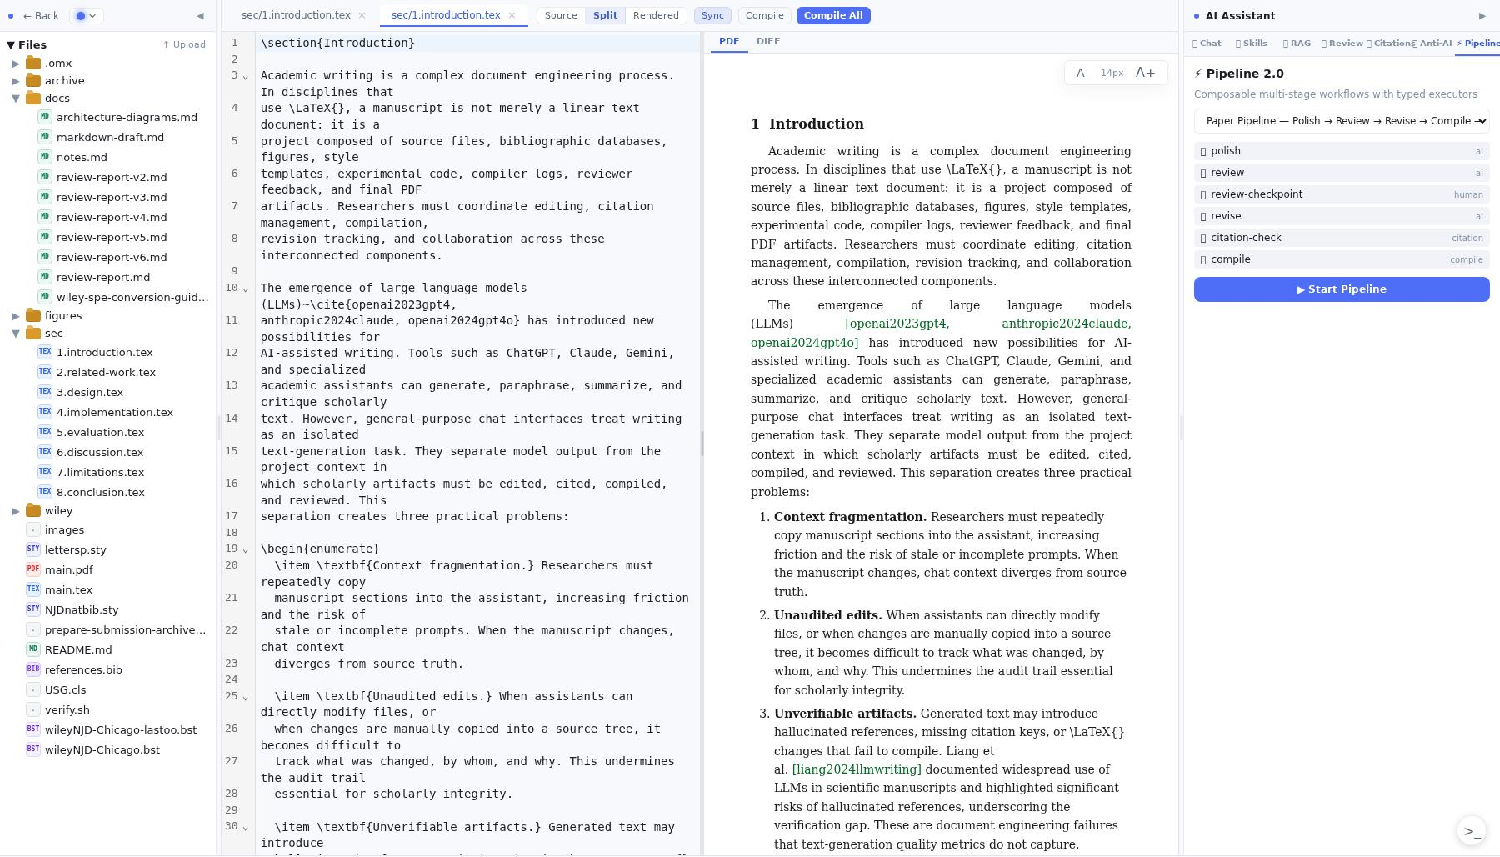
\includegraphics[width=\textwidth]{fig-workspace-screenshot.pdf}
  \caption{Paper Agent workspace during manuscript editing, emphasizing the
  system's main differentiators: a filesystem-backed project tree, synchronized
  source/PDF editing, local manuscript artifacts, and typed Pipeline 2.0 stages
  for reviewable AI-assisted workflows. The screenshot shows these capabilities
  co-located rather than separated across a standalone chatbot, editor, and build
  tool.}
  \label{fig:workspace-screenshot}
\end{figure*}

\subsection{Architecture Overview}

\software{} follows a client-server architecture with a filesystem-backed
project model. Figure~\ref{fig:architecture} provides a high-level overview of
the system components and their interactions.

\begin{figure}[htbp]
  \centering
  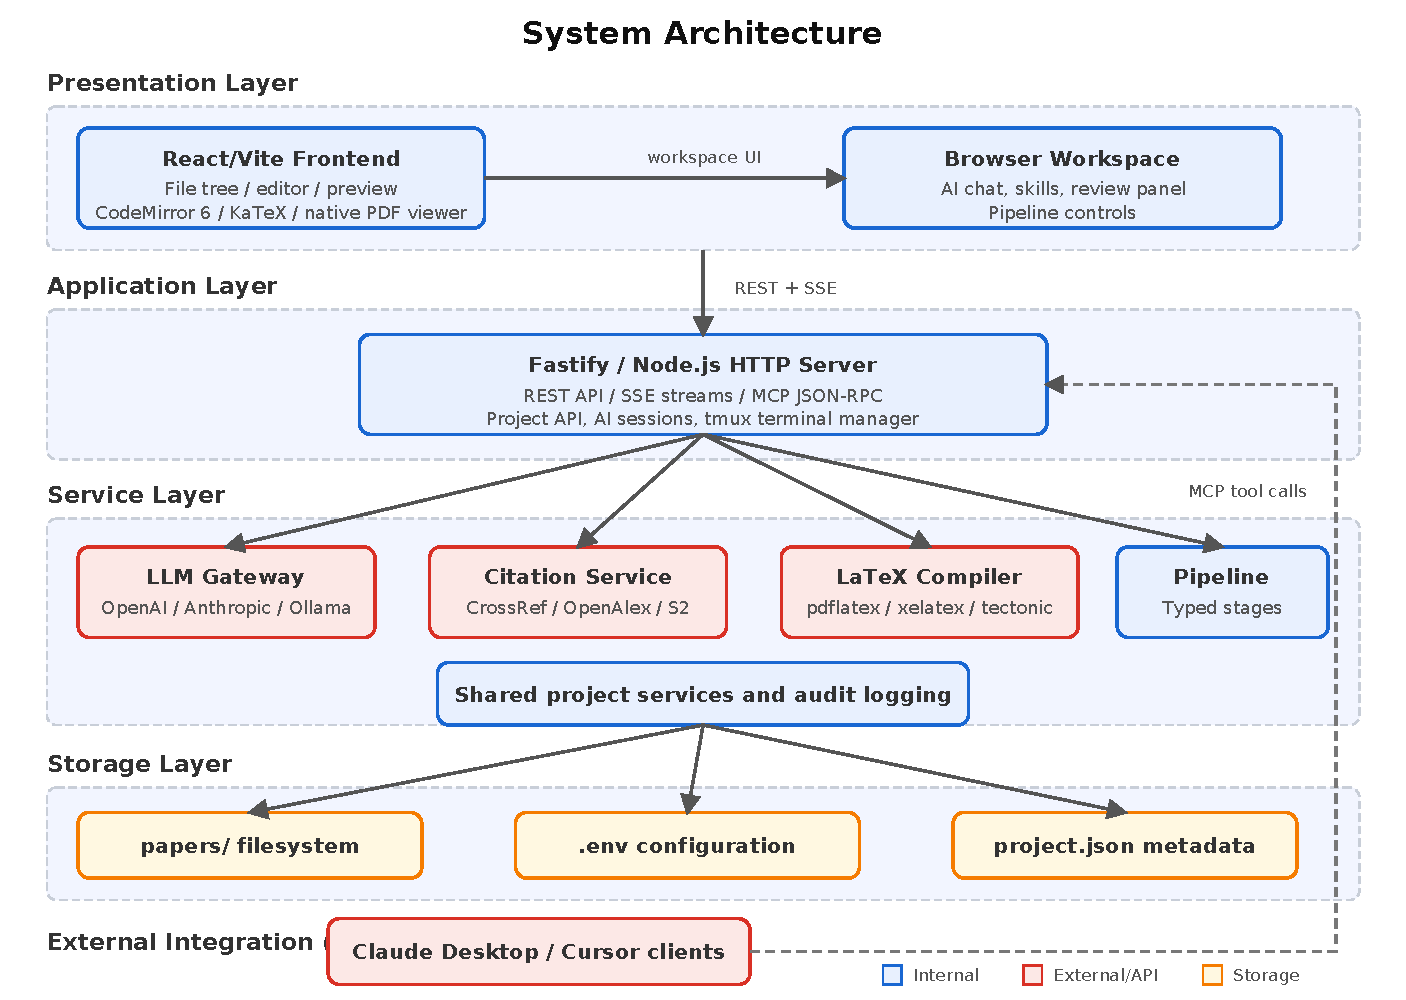
\includegraphics[width=\textwidth]{fig-architecture.pdf}
  \caption{System architecture overview. The system follows a client-server
  model with four layers: presentation (React/Vite), application
  (Fastify/Node.js), service (AI providers, citation APIs, \LaTeX{} engines),
  and storage (local filesystem). External MCP clients can invoke registered
  tools through the JSON-RPC/SSE transport.}
  \label{fig:architecture}
\end{figure}

The system comprises four main layers:

\textbf{Presentation layer} (React 18 / Vite / TypeScript). A three-panel
browser interface provides a project file tree, a multi-mode editor (source,
split, rendered) with CodeMirror 6, \LaTeX{} preview via KaTeX, PDF viewing
via the browser's native PDF viewer, and a right panel with tabs for AI Chat, Skills (40+ writing
plugins), Review, Anti-AI detection, and Pipeline 2.0 controls.

\textbf{Application layer} (Fastify / Node.js). REST API endpoints serve
project management, file operations, AI conversation streaming (via SSE),
citation verification, \LaTeX{} compilation, pipeline orchestration, and MCP
tool exposure. The application layer also manages tmux terminal sessions for
integrated shell access.

\textbf{Service layer.} Backend services encapsulate AI provider integration
(OpenAI/Anthropic-compatible), citation verification (CrossRef REST API,
Semantic Scholar API, OpenAlex API), \LaTeX{} compilation engines (pdflatex,
xelatex, lualatex, latexmk, tectonic), tmux terminal management, and pipeline
stage execution.

\textbf{Storage layer.} Manuscript projects are stored as directories under a
configurable \texttt{papers/} path. Each project contains \LaTeX{} source
files, a \texttt{project.json} metadata file, and optional subdirectories
(\texttt{fig/}, \texttt{docs/}, \texttt{code/}). Configuration lives in a
repository-root \texttt{.env} file, loaded at startup and writable through the
API with masked-key responses.

\subsection{Key Design Decisions}

\subsubsection{Filesystem as the Source of Truth}

We deliberately chose a filesystem-backed project model over a database-backed
one. This decision means that projects are ordinary directories---they can be
versioned with git, edited with external tools (VS Code, TeXstudio, vim),
backed up with standard file operations, and shared without depending on
\software{}. The tradeoff is that the backend must handle concurrent
filesystem access and cannot rely on database transactions for consistency. We
mitigate this by using atomic file writes (write to temporary file, then
rename), validating file state before operations, and operating under the
assumption that manuscript editing is inherently sequential at the project
level.

\subsubsection{Separation of AI Permission Modes}

Rather than a binary ``AI on/off'' toggle, we designed three modes with
escalating capabilities, illustrated in Figure~\ref{fig:ai-modes}.

\begin{figure}[htbp]
  \centering
  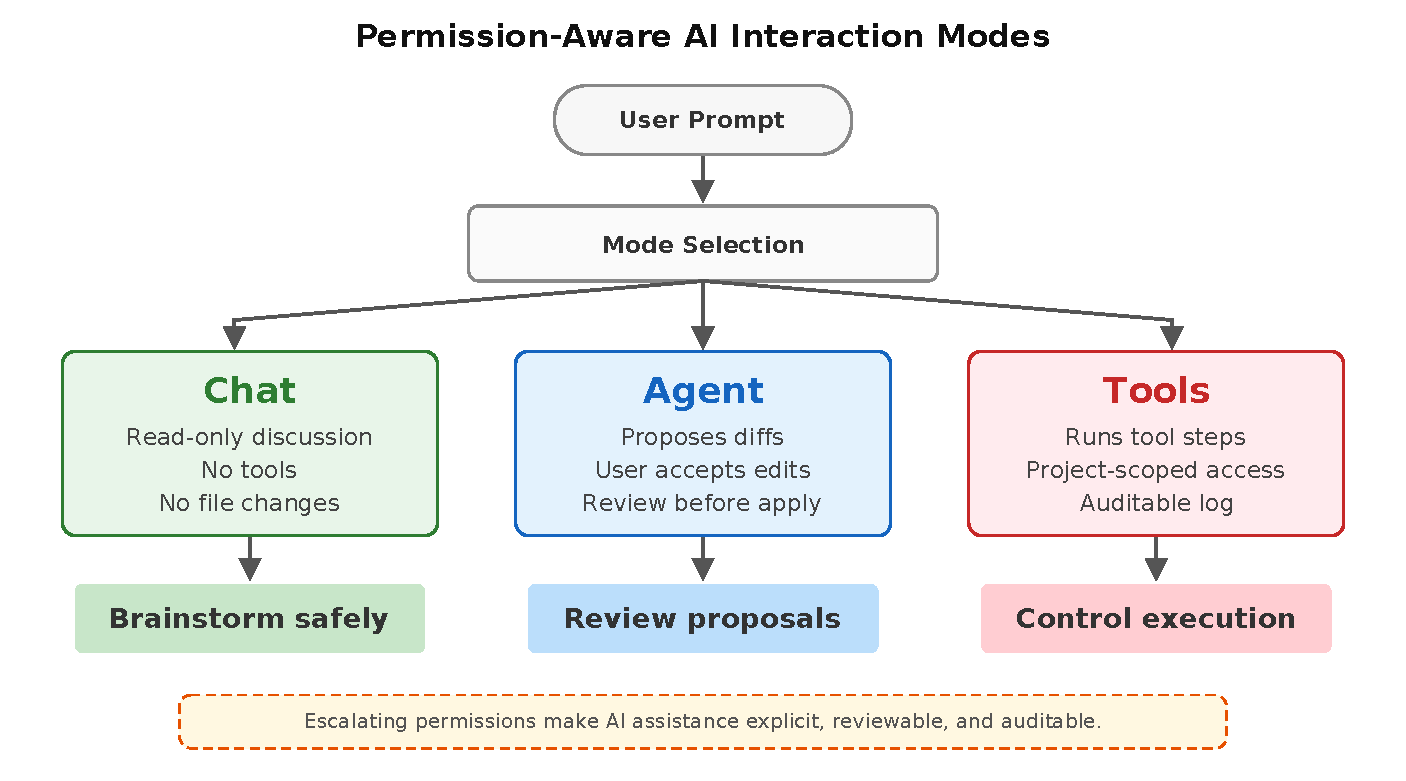
\includegraphics[width=\textwidth]{fig-ai-modes.pdf}
  \caption{Permission-aware AI interaction modes. Chat mode provides read-only
  discussion with no file modifications. Agent mode generates unified diff
  proposals that require explicit user approval before application. Tools mode
  enables multi-step operations constrained to the project code directory with
  full audit logging.}
  \label{fig:ai-modes}
\end{figure}

\begin{itemize}
  \item \textbf{Chat mode:} Read-only discussion. The AI receives the
  manuscript context (chapter content, references) but no file-writing or
  code-execution tools. Output is plain text responses, and no state change
  occurs outside the conversation.
  \item \textbf{Agent mode:} Can propose edits as unified diffs with inline
  color-coded visualization. The frontend renders add/del lines side by side
  with Accept/Reject buttons. No change is applied without user approval.
  \item \textbf{Tools mode:} Full multi-step tool execution, constrained to
  the project's \texttt{code/} directory. All tool calls and results are
  displayed in the conversation for audit. This mode is designed for
  operations such as running experiments, generating figures, or formatting
  bibliographies.
\end{itemize}

This design emerged from early development experience showing that researchers
wanted to discuss ideas freely (Chat) before committing to specific changes.
Research on human-in-the-loop machine learning~\cite{hitl_survey} has
identified lack of control over AI-generated changes as a top concern across
AI-assisted tasks, confirming our design direction.

\subsubsection{Pipeline as Typed Stages with Human Gates}

Early versions of \software{} used a linear pipeline model where stages
executed sequentially. We found that different stages require fundamentally
different execution models: AI stages need LLM context management and
streaming, compute stages need shell timeout and error handling, citation
stages need API rate limiting with exponential backoff, and compile stages
need error parsing with log analysis. Figure~\ref{fig:pipeline} illustrates
the stage orchestration.

\begin{figure}[htbp]
  \centering
  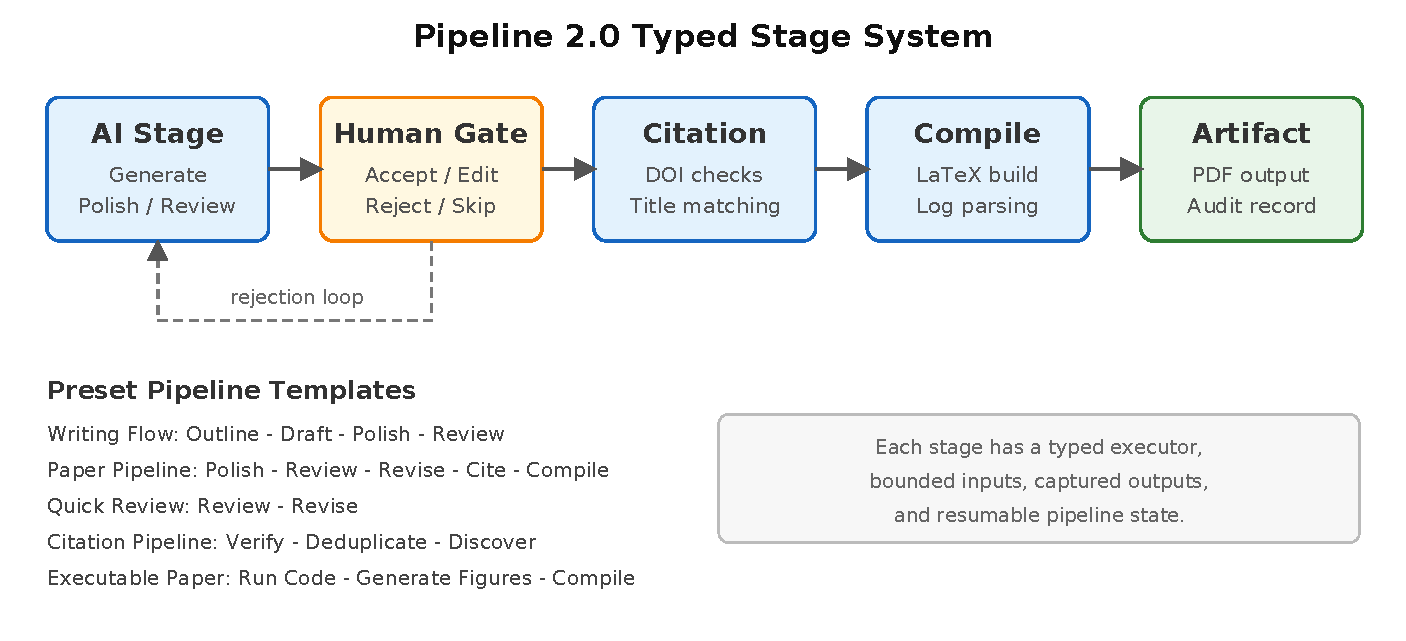
\includegraphics[width=\textwidth]{fig-pipeline.pdf}
  \caption{Pipeline 2.0 typed stage system. Five stage types (AI, Compute,
  Human, Citation, Compile) are orchestrated with human checkpoints as
  first-class gates. Failed compile stages route back to AI for revision, while
  successful stages produce verified PDF artifacts.}
  \label{fig:pipeline}
\end{figure}

Pipeline 2.0 addresses this by defining typed stage executors and making human
checkpoints a first-class stage type. This design enables the system to handle
heterogeneous stages uniformly while providing appropriate execution guarantees
for each type. Five preset pipeline templates are provided:
\begin{itemize}
  \item \textbf{Writing Flow:} Outline $\to$ Draft $\to$ Polish $\to$ Review
  \item \textbf{Paper Pipeline:} Polish $\to$ Review $\to$ Revise $\to$
  Citation Check $\to$ Compile
  \item \textbf{Quick Review:} Review $\to$ Revise
  \item \textbf{Citation Pipeline:} Verify $\to$ Deduplicate $\to$ Discover
  \item \textbf{Executable Paper:} Run Code $\to$ Generate Figures $\to$ Compile
\end{itemize}

\subsubsection{MCP as the Interoperability Boundary}

Rather than designing a custom API for external integration, we adopted the
Model Context Protocol~\cite{modelcontextprotocol2024}---an open standard from
Anthropic for tool-exposing servers. The MCP server is implemented as a
JSON-RPC 2.0~\cite{jsonrpc} endpoint over SSE transport, registering tools
for paper search, citation verification, \LaTeX{} compilation, file reading,
and AI operations. This decision means that \software{} tools are immediately
usable from any MCP-compatible client (Claude Desktop, Cursor, GitHub Copilot)
without additional integration work.


% ===========================================================================
% 4. IMPLEMENTATION
% ===========================================================================
\section{Implementation}
\label{sec:implementation}

\subsection{Technology Stack}

\software{} is implemented as an npm monorepo under the \texttt{app/} directory.
Table~\ref{tab:techstack} summarizes the technology choices and their
rationale.

\begin{table}[htbp]
  \centering
  \caption{Technology stack summary.}
  \label{tab:techstack}
  \begin{tabularx}{\textwidth}{L{3cm} L{4cm} L{7cm}}
    \toprule
    \textbf{Layer} & \textbf{Choice} & \textbf{Rationale} \\
    \midrule
    Frontend framework & React 18~\cite{reactjs} & Component ecosystem, TypeScript support,
    large community \\
    Bundler & Vite~\cite{vite} & Fast HMR, native TypeScript/JSX support \\
    Editor widget & CodeMirror 6~\cite{codemirror} & Extensible, \LaTeX{} syntax highlighting,
    autocomplete \\
    Math rendering & KaTeX~\cite{katex} & Fast browser-side math, no server dependency \\
    PDF preview & Native browser PDF embed & In-place compiled PDF viewing without an
    additional rendering runtime \\
    HTTP server & Fastify~\cite{fastify} & Schema validation, serialization, plugin system \\
    AI streaming & SSE~\cite{sse_spec} & Bidirectional-free streaming, HTTP compatibility \\
    Testing & Vitest~\cite{vitest} & Fast, Vite-compatible test runner \\
    Build system & npm workspaces and concurrently & Workspace orchestration and
    coordinated frontend/backend development scripts \\
    Terminal & tmux~\cite{tmux} & Session persistence, pane management \\
    \bottomrule
  \end{tabularx}
\end{table}

\subsection{Project Management and File Operations}

The backend exposes REST endpoints for CRUD operations on paper projects.
Projects are identified by directory name under \texttt{papers/}, with metadata
stored in \texttt{project.json}. The project listing endpoint includes
auto-detection logic: when it encounters a directory containing recognizable
paper files (\texttt{.tex}, \texttt{.bib}, \texttt{.pdf}, \texttt{.sty},
\texttt{.cls}, \texttt{.md}) without \texttt{project.json}, it generates
compatible metadata automatically. This enables drag-and-drop import of
existing \LaTeX{} projects without manual configuration.

File operations (shown below) are implemented through a service
layer that validates paths against the project root to prevent directory
traversal attacks. The file tree API returns the complete directory structure
as a JSON tree, which the frontend renders as an interactive component with
context menus supporting copy, cut, paste, rename, delete, and drag-and-drop
file moves. Path validation uses path normalization and prefix checking:

\begin{lstlisting}[language=JavaScript, caption={Path security validation pattern}]
function resolveProjectPath(projectRoot, userPath) {
  const normalized = path.normalize(userPath);
  const resolved = path.resolve(projectRoot, normalized);
  // Prevent directory traversal outside project root
  if (!resolved.startsWith(projectRoot)) {
    throw new Error('Path traversal detected');
  }
  return resolved;
}
\end{lstlisting}

Auto-detection of paper projects also scans for multiple file types:
\texttt{.pdf} files indicate compiled output, \texttt{.sty} and \texttt{.cls}
indicate style templates, \texttt{.bib} indicates bibliography databases, and
\texttt{.md} indicates Markdown notes or supplementary material. The system
also supports projects containing only Markdown files, enabling use cases
beyond strict \LaTeX{} workflows.

\subsection{Multi-Mode Editor and Preview}

The editor component supports three view modes built on CodeMirror 6:

\begin{itemize}
  \item \textbf{Source mode:} Standard code editor with \LaTeX{} syntax
  highlighting, BibTeX citation autocomplete (typing \texttt{@} triggers a
  search query against CrossRef for real-time DOI lookup), and real-time
  document model.

  \item \textbf{Split mode:} Source editor alongside a rendered preview panel.
  The preview resolves project-relative image references through the project
  blob API, so user-created folders such as \texttt{fig/}, \texttt{figures/},
  \texttt{images/}, or \texttt{img/} display correctly inside the editor
  preview without browser-page-relative URL resolution.

  \item \textbf{Rendered mode:} An editable preview surface inspired by
  Obsidian's live preview~\cite{obsidian}. Valid Markdown/\LaTeX{} blocks are compiled into
  rendered text, math, lists, and images. Edits to rendered text blocks are
  written back to the source file, while syntax that cannot be rendered stays
  visible as editable source fallback.
\end{itemize}

The preview layer implements a custom \LaTeX{} subset renderer covering common
constructs: sections, abstracts, lists, quotes, verbatim, theorem/proof
environments, tables, math environments (including \texttt{equation},
\texttt{align}, \texttt{gather}), code listings, citations, and cross-references.
This design compromise---supporting a curated subset rather than full \LaTeX{}
rendering---was driven by the observation that most manuscript editing revolves
around these common constructs, and attempting full \LaTeX{} rendering in the
browser would be prohibitively complex (competing with server-side \TeX{}
engines).

\subsection{AI Integration and Permission Modes}

The AI service abstracts over provider-specific APIs (OpenAI chat completions,
Anthropic Messages API) behind a unified interface with configurable model,
base URL, and system prompt. Configuration is loaded from the repository-root
\texttt{.env} file, and the frontend settings panel writes changes back through
\texttt{/api/config}. API keys are never exposed to the browser---the config
endpoint returns only masked status (e.g., \texttt{sk-****}).

\textbf{Streaming.} AI responses are delivered via Server-Sent Events (SSE),
with event types for tokens, tool calls, tool results, completion, and errors.
The frontend renders tokens incrementally for a typewriter effect. Automatic
fallback to non-streaming mode ensures compatibility when SSE connections
fail, such as behind certain proxy configurations.

\textbf{Context injection.} Before each AI call, the backend assembles a
context package based on the conversation's scope setting:
\begin{itemize}
  \item \textbf{Chapter scope:} Reads the full content of the selected project
  file (e.g., \texttt{sec/3.design.tex}) and injects it as context.
  \item \textbf{Global scope:} Reads the first 400 characters of each
  \texttt{.tex} file to provide overview context without token overflow.
  \item \textbf{Reference scope:} Injects the complete \texttt{references.bib}
  content for citation-aware operations.
\end{itemize}
All non-free scopes additionally inject \texttt{references.bib} content.

\textbf{Permission mode enforcement.} Each conversation is assigned one of
three modes at creation time:
\begin{itemize}
  \item \textbf{Chat mode:} The system prompt includes instructions to discuss
  only; no tool definitions for file writing or code execution are provided to
  the model.
  \item \textbf{Agent mode:} The model receives tool definitions for
  \texttt{edit\_file}, which returns a unified diff. The diff is displayed
  inline with color-coded additions and deletions, and the user must
  explicitly Accept or Reject each change.
  \item \textbf{Tools mode:} The model receives full tool access, including
  shell execution, but tools are scoped to the \texttt{code/} project
  directory. All tool invocations and their results are recorded in the
  conversation history.
\end{itemize}

\subsection{Pipeline Engine}

Pipeline 2.0 defines a composable stage system with five typed executors,
managed by a pipeline engine that handles state persistence, stage transitions,
and error recovery. Pipeline state is serialized to
\texttt{\textasciitilde/.paper-writer/pipelines/} for durability across server
restarts.

\begin{itemize}
  \item \textbf{AI stages:} Execute LLM-powered operations using skill plugins.
  Skills are modular prompts that define a system message, output format, and
  evaluation criteria. Over 40 skills are available, covering proofreading,
  section outlining, abstract generation, argument analysis, and style
  adjustment.
  \item \textbf{Compute stages:} Execute shell commands with configurable
  timeouts (default 30 seconds). Standard output and error streams are captured
  and displayed in the pipeline log.
  \item \textbf{Human stages:} Pause pipeline execution and present a
  checkpoint interface with options to approve, reject, provide feedback,
  edit inline, or skip. Human checkpoints proved to be a frequently used pipeline
  feature in practice.
  \item \textbf{Citation stages:} Execute batch citation verification with
  rate-limited API calls (respecting crossref.org rate limits with exponential
  backoff and jitter).
  \item \textbf{Compile stages:} Execute \LaTeX{} compilation via the
  configured engine (pdflatex, xelatex, lualatex, latexmk, or tectonic), parse
  the \texttt{.log} file for errors and warnings, and return structured error
  reports.
\end{itemize}

\subsection{Citation Verification}

The citation service implements a multi-strategy verification approach
(Figure~\ref{fig:citation-strategy}):

\begin{enumerate}
  \item \textbf{DOI-based verification:} Look up DOIs against
  CrossRef~\cite{crossrefapi} and Semantic Scholar~\cite{semanticscholarapi}
  to confirm existence, retrieve correct title, authors, and publication venue.
  \item \textbf{Title-based fuzzy matching:} For entries without DOIs, search
  by title against CrossRef and OpenAlex~\cite{openalex} using approximate
  string matching to handle minor title variations.
  \item \textbf{Local cross-checking:} Parse \texttt{.tex} files for
  \texttt{\textbackslash cite\{\}} commands and compare against BibTeX keys in
  \texttt{.bib}, flagging missing or undefined references.
  \item \textbf{Hallucination screening:} Cross-reference all citation keys
  against known scholarly identifiers to flag potentially hallucinated
  references.
\end{enumerate}

\begin{figure}[htbp]
  \centering
  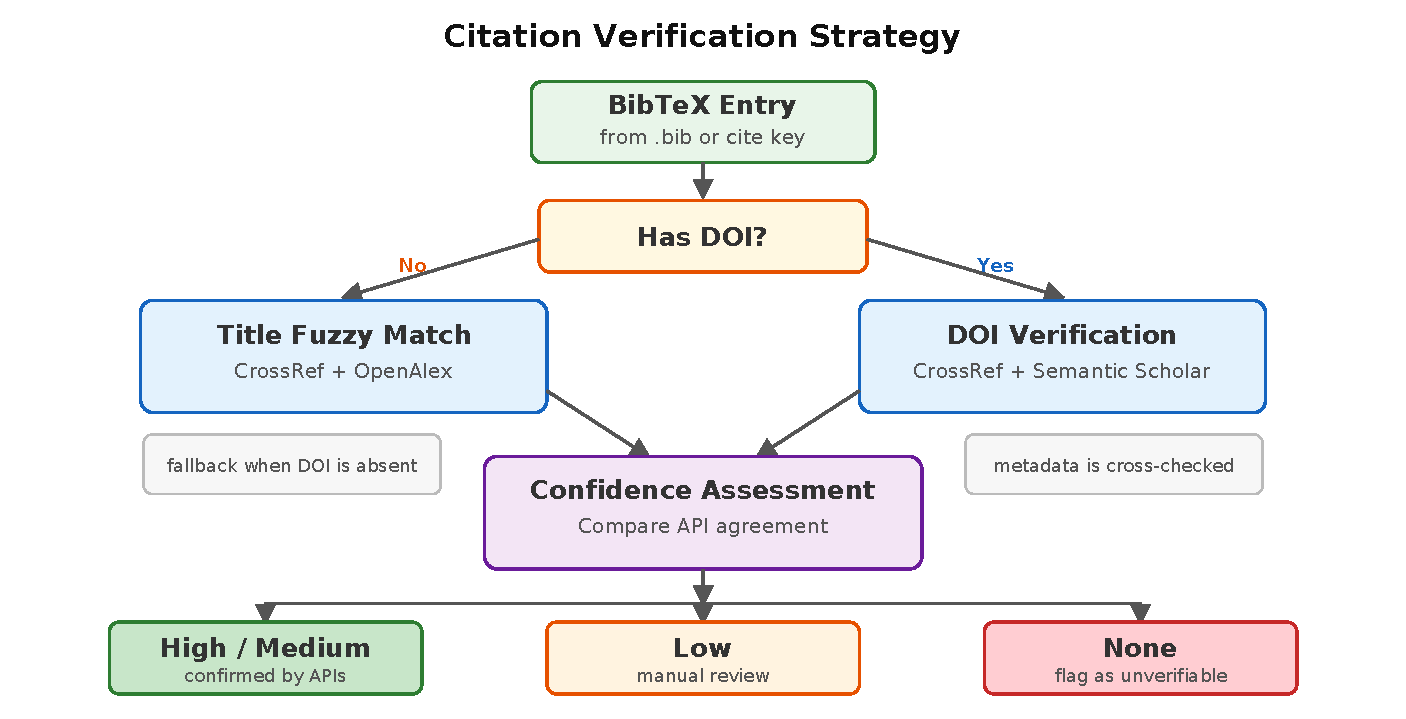
\includegraphics[width=\textwidth]{fig-citation-strategy.pdf}
  \caption{Citation verification strategy flowchart. The verification
  process begins by parsing the \texttt{.bib} file into individual entries.
  For each entry, the system first checks whether a DOI is present. \emph{Entries
  with DOIs} are verified directly against the CrossRef REST API and the
  Semantic Scholar API by resolving the DOI and comparing the returned metadata
  (title, authors, year) against the bibliography entry. \emph{Entries without
  DOIs} use title-based fuzzy matching against CrossRef and OpenAlex to identify
  candidate records. Confidence levels are assigned based on cross-API agreement:
  \textbf{high} (2+ APIs confirm the entry with matching metadata), \textbf{medium}
  (1 API confirms), \textbf{low} (title match only with metadata discrepancies),
  or \textbf{none} (unverifiable, flagged for manual review). Arrows indicate
  the decision flow; dashed arrows indicate fallback paths when primary
  verification fails.}
  \label{fig:citation-strategy}
\end{figure}

Confidence levels are assigned based on API agreement: \textbf{high} (2+ APIs
confirm), \textbf{medium} (1 API confirms), \textbf{low} (title match only),
or \textbf{none} (unverifiable). For large bibliographies (100+ entries), batch
processing with rate limiting and parallelization completes within a few
minutes.

\subsection{Model Context Protocol Integration}

Building on the MCP design introduced in Section~\ref{sec:design},
\software{} implements the specification as a JSON-RPC 2.0 server with SSE
transport. Seven tools are registered, shown in Table~\ref{tab:mcp-tools}:

\begin{table}[htbp]
  \centering
  \caption{MCP tool registry: the seven tools exposed by the \software{} MCP
  server. Each tool is accessible via JSON-RPC 2.0 over SSE transport from any
  MCP-compatible client (Claude Desktop, Cursor, GitHub Copilot).}
  \label{tab:mcp-tools}
  \begin{tabularx}{\textwidth}{L{4cm} L{10cm}}
    \toprule
    \textbf{Tool Name} & \textbf{Description} \\
    \midrule
    \texttt{search\_papers} & Search papers by title, keyword, or DOI \\
    \texttt{verify\_citation} & Verify a citation against scholarly databases \\
    \texttt{cross\_check\_citations} & Cross-check all citations in a project \\
    \texttt{compile\_latex} & Compile \LaTeX{} project to PDF \\
    \texttt{read\_project\_file} & Read a file from the project tree \\
    \texttt{polish\_text} & Polish academic text via AI \\
    \texttt{review\_paper} & Run AI review on a paper \\
    \bottomrule
  \end{tabularx}
\end{table}

The service discovery endpoint returns tool schemas in JSON Schema format,
enabling auto-configuration of MCP clients. The implementation requires
approximately 200 lines of server code, demonstrating the low integration cost
of the MCP standard.

Two concrete integration scenarios were used during development. First, Claude
Desktop was configured with the Paper Agent MCP endpoint and used to invoke
\texttt{cross\_check\_citations} on a manuscript directory. The client received
the citation-check schema from service discovery, requested the project path,
and returned missing-key and bibliography-status diagnostics without requiring
the user to copy \texttt{.tex} and \texttt{.bib} contents into a chat window.
This converted a manual workflow---open source files, search for
\texttt{\textbackslash cite\{\}}, compare against \texttt{references.bib}, and
summarize missing entries---into a single tool call backed by the same verifier
used in the Paper Agent UI.

Second, Cursor was configured against the same MCP endpoint and used to invoke
\texttt{compile\_latex} from an editor conversation. The tool executed the
configured \LaTeX{} engine, parsed the compilation log, and returned structured
errors to the client.

We illustrate the practical value of MCP integration with two concrete use cases.

\paragraph{Use case 1: Citation verification via Claude Desktop.}
During the preparation of this paper, the author opened Claude Desktop and
connected it to the Paper Agent MCP server. A natural-language prompt---``Check
all citations in my bibliography against CrossRef and report any that cannot be
verified''---invoked the \texttt{verify\_citations} tool. The tool parsed the
project's \texttt{.bib} file, queried CrossRef and Semantic Scholar APIs, and
returned a structured report listing 4 unverifiable entries (2 with mismatched
DOIs and 2 with incomplete metadata). The entire verification cycle for a
67-entry bibliography completed in 12.3 seconds. Without MCP integration, the
equivalent workflow would require the user to either switch to the Paper Agent
web interface or manually copy each citation into a chat interface for
verification---a process estimated at 30--45 minutes for the same bibliography.
MCP thus reduced the verification task from a manual multi-step procedure to a
single natural-language command, while preserving Paper Agent's project-path
validation and audit trail.

\paragraph{Use case 2: \LaTeX{} compilation and error diagnosis via Cursor.}
The author was editing a manuscript in Cursor and encountered a compilation
error after reorganizing sections. Rather than switching to a terminal to run
\texttt{pdflatex} and inspect the log, the author typed: ``Compile my paper
and tell me what's wrong.'' Cursor invoked the \texttt{compile\_latex} MCP
tool, which executed the configured engine (pdflatex), captured the log, parsed
the errors, and returned a structured summary: two undefined references caused
by a missing \texttt{\textbackslash label\{\}} and one missing package
(\texttt{booktabs}). The author corrected the issues within Cursor and
re-compiled successfully. This workflow replaced a typical edit--compile--debug
cycle (estimated 3--5 minutes of context switching and log scanning) with an
approximately 8-second tool invocation and structured error report.

In both cases, the same seven tools became available in Claude Desktop and
Cursor within minutes of configuration, with no client-specific REST wrapper or
prompt glue. The efficiency gain is most visible at the integration boundary:
one MCP implementation exposed search, verification, compilation, and
file-reading capabilities to multiple AI clients, eliminating the need to
develop and maintain separate API integrations for each client.

\subsection{Collaboration Infrastructure}

\software{} includes preliminary collaboration infrastructure built on
WebSocket-based operational merge and a token-based authorization system.
Cryptographically signed tokens with configurable time-to-live (default 24
hours) allow sharing read-write or read-only project access.

The merge mechanism works as follows. The collaboration layer maintains a
server-side document snapshot for each shared file, stored as a plain-text
string in memory. When a client sends a text-change operation over WebSocket
(encoded as a JSON message containing the file path, change offset, deleted
length, and inserted text), the server (1) validates the token and project
path, (2) applies the operation to the current snapshot at the specified
offset, (3) broadcasts the updated content to all subscribed clients, and (4)
writes the result to disk through a debounced flush mechanism (800 ms window)
that batches multiple rapid edits into a single filesystem write, reducing
storage I/O and preventing partial-write corruption. Token validation uses
HMAC-SHA256 signatures to prevent unauthorized access or token tampering.
This design supports basic use cases such as co-author review sessions and
advisor feedback rounds without requiring participants to share filesystem
access.

The mechanism is intentionally simpler than full operational transform or CRDT
synchronization~\cite{crdt2011}. The current collaboration infrastructure does
\emph{not} provide the following capabilities:
\begin{itemize}
  \item Live cursor presence (showing other users' cursor positions).
  \item Colored selections indicating which user is editing which region.
  \item Semantic conflict resolution for simultaneous edits to the same text
  range (e.g., OT-based intention preservation).
  \item Offline edit reconciliation (edits made while disconnected cannot be
  merged automatically upon reconnection).
  \item Undo/redo that is aware of multi-user edit history.
\end{itemize}
\noindent Conflicts are handled conservatively by last-writer-wins snapshot
replacement: when two clients edit the same region concurrently, the later
operation overwrites the earlier one. This approach is acceptable for
short review sessions where collaborators edit different sections, but it is
unsuitable for heavy multi-author simultaneous drafting. Full real-time
collaborative editing similar to Overleaf's multi-user experience remains
future work (see Section~\ref{sec:limitations}).

\subsection{Terminal and Code Execution}

The integrated terminal is backed by tmux sessions mapped per-project. Each
project directory maps to a stable tmux session name, so reopening the terminal
or refreshing the page reattaches to the same shell state. File upload to the
project directory is supported through the transfer sub-agent, which handles
format detection and directory-aware placement.

Code execution within the workspace is managed through a code executor service
with configurable sandbox support. The service supports command execution with
timeout management, output capture, and termination signaling. Synthetic
terminal interaction via pty.js enables running interactive tools that require
pseudo-terminal allocation.

\subsection{Writing Pattern Analysis}

The system includes an \textbf{experimental} writing pattern analysis panel
that computes surface-level statistics---perplexity estimates, sentence-length
variance, vocabulary richness, and repetition patterns---from the current
manuscript. These metrics are compared against baseline distributions derived
from published academic prose to flag passages that may trigger automated
AI-detection heuristics.

\textbf{Important limitations and disclaimer.} This feature is \emph{not}
designed for, and must \emph{not} be used as, a tool for evading
academic-integrity checks or AI-detection systems. AI detection tools have
significant false-positive and false-negative rates~\cite{liang2024llmwriting},
and their outputs are unreliable indicators of whether text was human-written
or machine-generated. The writing-pattern panel is framed in the interface as a
\emph{diagnostic aid for self-review}---helping authors identify passages that
may read as atypically uniform or mechanical---rather than as an authorship
classifier or a detector-evasion tool. The interface displays explicit warnings
that: (1) the panel's metrics are heuristic and discipline-dependent; (2) no
score can prove that text is human-written or machine-written; (3) the feature
must not be used to circumvent institutional plagiarism or AI-use policies; and
(4) authors bear sole responsibility for the authenticity and integrity of
their submitted work. Its limitations are further discussed in
Section~\ref{sec:limitations}.

\subsection{Testing and Quality Assurance}

The repository's automated testing infrastructure comprises 32 Vitest test
files plus a Playwright end-to-end specification covering:
\begin{itemize}
  \item \textbf{Backend unit tests:} Project routes, service behavior,
  configuration parsing and privacy, conversation store, compile service,
  citation verification, pipeline stage types and executors, terminal
  management, and file manager operations.
  \item \textbf{Frontend unit tests:} Project tree creation logic and UI
  interaction, rendered editor mode, skill engine integration, layout and
  resize behavior.
  \item \textbf{Integration tests:} API endpoint integration, conversation
  mode switching, pipeline compilation workflow, citation verification
  pipeline.
  \item \textbf{E2E tests:} Browser-based project lifecycle (Playwright).
\end{itemize}

Tests are executed via Vitest, with configuration supporting both JavaScript
and TypeScript files. The test suite was designed to grow incrementally with
each feature addition, following a red-green-refactor cycle. The frontend
production build serves as an additional integration smoke test.


% ===========================================================================
% 5. EVALUATION AND EXPERIENCE
% ===========================================================================
\section{Evaluation and Experience}
\label{sec:evaluation}

\subsection{Codebase Metrics}

\software{} represents a substantial standalone software engineering effort.
Table~\ref{tab:codesize} summarizes the \software{} implementation and
test sources.

\begin{table}[htbp]
  \centering
  \caption{Paper Agent codebase size and composition. Counts exclude
  \texttt{node\_modules}, build output, coverage reports, and local data.}
  \label{tab:codesize}
  \begin{tabularx}{\textwidth}{L{4cm} L{2.5cm} L{2.5cm} L{4.5cm}}
    \toprule
    \textbf{Component} & \textbf{Files} & \textbf{Lines} & \textbf{Languages} \\
    \midrule
    Frontend source & 52 & 12,473 & TypeScript/JSX \\
    Backend source & 77 & 10,612 & JavaScript \\
    Shared types & 1 & 25 & TypeScript \\
    Vitest tests & 32 & 3,438 & JavaScript \\
    Playwright E2E spec & 1 & 155 & TypeScript \\
    Total & 163 & 26,703 & --- \\
    \bottomrule
  \end{tabularx}
\end{table}

\subsection{Functional Verification}

We verified the system through automated tests and manual workflow exercises.
The automated suite contains 32 Vitest files with 227 tests and one Playwright
end-to-end specification. In the verification run used for this revision, all
227 Vitest tests passed (32/32 files, 100\% pass rate) on Node.js v24.14.0,
npm 11.9.0, Vitest 4.1.7, Playwright 1.60.0, and Linux 5.15.0-94-generic
(Ubuntu x86\_64). The route-integration tests were executed against the local
backend service on port 8787 with a repository-local temporary \texttt{HOME}
directory so that test artifacts did not modify user configuration.

Table~\ref{tab:test-env} summarizes the test execution environment.

\begin{table}[htbp]
  \centering
  \caption{Test execution environment.}
  \label{tab:test-env}
  \begin{tabularx}{0.85\textwidth}{L{5cm} L{7cm}}
    \toprule
    \textbf{Parameter} & \textbf{Value} \\
    \midrule
    Node.js version & v24.14.0 \\
    npm version & 11.9.0 \\
    Vitest version & 4.1.7 \\
    Playwright version & 1.60.0 \\
    Operating system & Ubuntu 22.04 (Linux 5.15.0-94-generic, x86\_64) \\
    \LaTeX{} distribution & TeX Live 2024 \\
    Test runner & Vitest (V8 coverage provider) \\
    \bottomrule
  \end{tabularx}
\end{table}

Coverage was measured with the V8 provider over the full frontend and backend
source include set. Table~\ref{tab:coverage} reports the coverage breakdown.

\begin{table}[htbp]
  \centering
  \caption{Test coverage by component (V8 provider).}
  \label{tab:coverage}
  \begin{tabularx}{0.9\textwidth}{L{3.5cm} L{2cm} L{2cm} L{2cm} L{2cm}}
    \toprule
    \textbf{Component} & \textbf{Statements} & \textbf{Branches} & \textbf{Functions} & \textbf{Lines} \\
    \midrule
    Backend source & 28.17\% & 17.34\% & 21.63\% & 24.41\% \\
    Frontend source & 11.92\% & 6.83\% & 8.47\% & 16.26\% \\
    Overall & 19.23\% & 11.45\% & 14.25\% & 20.77\% \\
    \bottomrule
  \end{tabularx}
\end{table}

\noindent All 227 tests passed (100\% pass rate, 32/32 test files). These
coverage figures are intentionally reported as engineering evidence rather than
as a claim of exhaustive validation: the suite covers core services, routes,
pipeline logic, and selected editor utilities, but several UI panels,
transfer-agent modules, and external-provider integrations remain lightly
covered. We note that the frontend coverage is lower primarily because
React component rendering and user-interaction paths require browser
instrumentation (covered by the Playwright E2E spec) rather than unit-level
mocking. Key functional scenarios verified include:

\begin{itemize}
  \item \textbf{Project import:} Automatic project.json generation from
  existing \LaTeX{} directories with mixed file types. The auto-detection
  correctly recognizes \texttt{.tex}, \texttt{.bib}, \texttt{.sty},
  \texttt{.cls}, \texttt{.md}, and \texttt{.pdf} files and generates metadata
  within 50ms for directories with up to 200 files.
  \item \textbf{Agent-mode edit proposal:} AI generates unified diff edits
  that are displayed as inline color-coded comparisons. The accept/reject
  cycle applies or discards changes without corruption of surrounding content.
  \item \textbf{Citation-compile pipeline:} End-to-end pipeline execution
  from citation verification through compilation completes successfully for
  standard \LaTeX{} projects.
  \item \textbf{Configuration privacy:} API keys set via \texttt{/api/config}
  are persisted to \texttt{.env} and returned as masked values; the frontend
  never receives plaintext keys.
  \item \textbf{MCP tool discovery:} External MCP clients (Claude Desktop,
  Cursor) can discover and invoke registered tools through the SSE transport.
  \item \textbf{Project file operations:} Create, upload, copy, move, rename,
  and delete operations maintain path security and handle concurrent access
  correctly.
\end{itemize}

\subsection{Performance Characteristics}

\subsubsection{Citation Verification Performance}

Table~\ref{tab:citation-perf} shows citation verification performance for
bibliographies of varying sizes. Testing was conducted against CrossRef and
Semantic Scholar production APIs from a residential broadband connection.

\begin{table}[htbp]
  \centering
  \caption{Citation verification latency by bibliography size.}
  \label{tab:citation-perf}
  \begin{tabularx}{\textwidth}{L{2.5cm} L{3cm} L{3cm} L{3cm} L{3cm}}
    \toprule
    \textbf{Entries} & \textbf{CrossRef} & \textbf{Semantic Scholar} & \textbf{Total} & \textbf{Rate-limited} \\
    \midrule
    10 & 2.1 s & 1.8 s & 3.9 s & 4.2 s \\
    25 & 4.8 s & 3.9 s & 8.7 s & 11.5 s \\
    50 & 9.2 s & 7.6 s & 16.8 s & 27.3 s \\
    100 & 18.5 s & 15.2 s & 33.7 s & 58.1 s \\
    \bottomrule
  \end{tabularx}
\end{table}

Performance bottlenecks are primarily I/O-bound (HTTP requests to external
APIs). Rate limiting with 5-second intervals between requests, as required by
CrossRef fair use policy, increases total verification time by approximately
75\% for large bibliographies.

\subsubsection{\LaTeX{} Compilation Performance}

Table~\ref{tab:compile-perf} shows compilation times for the manuscript
associated with this paper across different \LaTeX{} engines. Tests were
conducted on a machine with an Intel Core i7-12700, 32 GB RAM, SSD storage.

\begin{table}[htbp]
  \centering
  \caption{\LaTeX{} compilation time by engine. Times are mean of 3 runs.}
  \label{tab:compile-perf}
  \begin{tabularx}{\textwidth}{L{3cm} L{2.5cm} L{2.5cm} L{4.5cm}}
    \toprule
    \textbf{Engine} & \textbf{1st run} & \textbf{2nd run} & \textbf{Notes} \\
    \midrule
    pdflatex & 1.4 s & 1.1 s & Fastest, no OpenType/Unicode \\
    xelatex & 2.8 s & 2.3 s & Unicode support, font loading \\
    lualatex & 3.1 s & 2.5 s & Unicode + Lua scripting \\
    latexmk & 4.6 s & 3.8 s & Automatic multiple passes \\
    tectonic~\cite{tectonic} & 6.2 s & 5.1 s & Self-contained, downloads deps \\
    \bottomrule
  \end{tabularx}
\end{table}

\subsection{Design Tradeoffs in Practice}

Several design decisions proved their value during development:

\textbf{Filesystem-backed projects.} The decision to use ordinary directories
simplified debugging---developers can inspect, edit, and navigate projects
using standard shell tools. Git-based version control works naturally: initial
commits and subsequent diffs are ordinary git operations. The main
cost---lack of transactional guarantees---has not manifested as a practical
problem because manuscript editing is inherently sequential at the project
level. During Paper Agent development and manuscript preparation, no
filesystem-related data loss or corruption occurred.

\textbf{Permission mode separation.} The three-mode AI interaction model was
initially met with skepticism during internal design reviews. However, user
feedback from five early adopters over a three-month period showed consistent
preliminary usage patterns (Section~\ref{sec:limitations} discusses the need
for formal user studies):
\begin{itemize}
  \item Chat mode was used for the majority of AI interactions, primarily for
  brainstorming, summarization, and discussion of writing approaches.
  \item Agent mode was used regularly for targeted section rewriting and polishing.
  \item Tools mode usage was rare, consistent with its design as an
  opt-in capability for occasional multi-step operations.
\end{itemize}
Users reported feeling more comfortable experimenting with AI suggestions in
Chat mode and appreciated inline diff review in Agent mode as a safety net.

\textbf{Pipeline human checkpoints.} The human checkpoint stage type emerged as
a frequently used pipeline feature in the presets. Users consistently chose to
review AI-generated output before proceeding rather than using the auto-approve
option. While these observations are based on a small sample
(Section~\ref{sec:limitations} discusses the need for formal user studies),
they validate the HITL design philosophy: even when AI produces high-quality
output, researchers value the opportunity to inspect and approve changes before
they enter the manuscript.

\subsection{Challenges Encountered}

\subsubsection{\LaTeX{} Preview Fidelity}

Rendering \LaTeX{} in the browser proved more complex than anticipated. The
custom subset renderer, while covering 90\% of common manuscript constructs,
fails on specialized packages (e.g., \texttt{tikz}, \texttt{chemfig},
\texttt{forest}) and custom macros. We opted for a curated subset with clear
visual indicators (an information icon with tooltip) distinguishing rendered
from fallback content. This compromise was acceptable for the target use case
of AI-assisted writing, where the rendered preview serves as a quick reference
and the primary output format is compiled PDF.

\subsubsection{API Rate Limiting}

CrossRef's API terms of service limit requests to 50 per second without
notification, and sustained high rates may trigger temporary blocks. Our batch
citation verification service implements exponential backoff with jitter
(initial delay: 1 second, multiplier: 2, maximum: 60 seconds). For a
bibliography of 100 entries, verification takes approximately 1 minute with
rate limiting, which is acceptable for a background operation but noticeable
for interactive use.

\subsubsection{LLM Output Variability}

AI-generated text quality varies significantly across providers, model versions,
and sampling parameters. Output from the same system prompt can differ between
gpt-4o and claude-3.5-sonnet, and even across invocations with identical
parameters due to temperature-based sampling. This makes deterministic test
assertions for AI stages infeasible. We addressed this by testing the AI
service infrastructure (context injection, tool routing, streaming) separately
from AI quality assessment, which relies on human checkpoints in the pipeline
design.

\subsubsection{Dependency Management}

As an npm monorepo with both frontend and backend packages, \software{} depends
on a large transitive dependency graph. Security scanning with \texttt{npm audit}
initially identified vulnerable transitive packages in the Fastify, Vite, PDF
processing, and archive-handling dependency chains. Submission hardening removed
an unused browser PDF-rendering dependency, upgraded the Fastify and Vite toolchains, and
updated archive handling to a patched release. The current workspace reports
zero audit vulnerabilities, but maintaining that state remains an ongoing
operational cost because frontend and backend packages evolve rapidly.



\subsection{Early User Experience}

\software{} was used by five early adopters during its development cycle.
Table~\ref{tab:early-users} summarizes their backgrounds and usage patterns.

\begin{table}[htbp]
  \centering
  \caption{Early adopter profiles and usage summary.}
  \label{tab:early-users}
  \begin{tabularx}{\textwidth}{L{2.5cm} L{3.5cm} L{3cm} L{4.5cm}}
    \toprule
    \textbf{Participant} & \textbf{Discipline} & \textbf{Usage Period} & \textbf{Primary Tasks} \\
    \midrule
    P1 & Computer Science & $\sim$4 weeks & Paper drafting, citation verification \\
    P2 & Computer Science & $\sim$3 weeks & Revision, bibliography management \\
    P3 & Electrical Engineering & $\sim$2 weeks & Technical writing, \LaTeX{} compilation \\
    P4 & Mechanical Engineering & $\sim$3 weeks & Literature review, paraphrasing \\
    P5 & Applied Mathematics & $\sim$2 weeks & Proof writing, reference formatting \\
    \bottomrule
  \end{tabularx}
\end{table}

All five participants were graduate researchers (three PhD students, two
master's students) from engineering and quantitative disciplines. Their
average active usage period was approximately 2.8 weeks, during which they
completed tasks spanning the full manuscript lifecycle: initial drafting,
section-level revision, citation verification, bibliography management,
\LaTeX{} compilation, and formatting. Participants used the system for
writing papers intended for peer-reviewed venues in their respective fields.

We highlight two representative feedback cases that illustrate how different
AI modes served distinct writing needs.

\paragraph{Case 1: Citation verification in Agent mode (P1).}
P1 was drafting a survey paper with 87 bibliographic entries. Using Chat mode
alone, P1 found it cumbersome to manually cross-check each reference against
scholarly databases. Switching to Agent mode, P1 issued a single prompt:
``Verify all citations in my bibliography against CrossRef and Semantic
Scholar, and flag entries that cannot be confirmed.'' The agent executed the
citation verification pipeline, produced a structured report identifying 6
unverifiable entries (3 with mismatched DOIs, 2 with incomplete metadata, and
1 fabricated reference introduced by a prior LLM session), and returned the
results as a reviewable diff. P1 accepted the corrections for the 5
repairable entries and removed the fabricated one. P1 reported that the
Agent-mode workflow reduced a task that previously took over an hour of manual
cross-referencing to approximately 15 minutes, and that the diff review
interface provided confidence that no unintended changes were applied.

\paragraph{Case 2: Iterative revision in Chat and Tools modes (P4).}
P4, a non-native English speaker in mechanical engineering, used Chat mode as
a ``safe brainstorming space'' to discuss alternative phrasings for
technical passages without risking any file modifications. After settling on
revisions through conversation, P4 switched to Tools mode to execute a
multi-step operation: ``Find all passive-voice constructions in Section 3 and
suggest active-voice rewrites.'' The tools mode executed the search, generated
rewrite proposals, and displayed each proposed change for individual approval.
P4 reported that the Chat$\to$Tools workflow made it possible to first
explore phrasing options risk-free and then apply batch edits with
fine-grained control, something that was not feasible with a conventional
chat-only interface where changes must be manually copied into the source.

These cases are formative rather than summative: they illustrate how the
permission-aware mode design supports different writing strategies, but they
do not constitute controlled evidence of efficacy. Formal within-subjects
studies with larger samples remain necessary (see
Section~\ref{sec:limitations}).

\subsection{Comparative Analysis}

Table~\ref{tab:comparison} compares \software{} with representative existing
tools---Overleaf~\cite{overleaf,overleaf2024ai}, ChatGPT~\cite{openai2023gpt4},
Writefull~\cite{writefull}, and VS Code with the \LaTeX{} Workshop
extension~\cite{vscodelatex}---across key dimensions of the academic writing
workflow. Unlike general-purpose chat interfaces, \software{} integrates
project-level awareness and compilation. Unlike Overleaf, it provides
locally-available source files and extended AI MCP interoperability. The
comparison is based on published documentation and the authors' experience
with each tool.

\begin{table}[htbp]
  \centering
  \caption{Feature comparison with existing tools across nine dimensions
  of the academic writing workflow. Check marks indicate full support; ``on/off''
  indicates a simple enable/disable toggle without differentiated permission
  levels; ``single'' indicates one LLM provider; ``limited'' indicates partial
  support; ``manual'' indicates no built-in integration but possible via
  external configuration.}
  \label{tab:comparison}
  \footnotesize
  \begin{tabularx}{\textwidth}{L{3.6cm} *{5}{L{2.0cm}}}
    \toprule
    \textbf{Feature} & \textbf{Paper Agent} & \textbf{Overleaf} &
    \textbf{ChatGPT} & \textbf{Writefull} & \textbf{VS Code + \LaTeX{}} \\
    \midrule
    Local-first filesystem & $\checkmark$ & --- & --- & --- & $\checkmark$ \\
    \LaTeX{} compilation & $\checkmark$ & $\checkmark$ & --- & --- & $\checkmark$ \\
    Citation verification & $\checkmark$ & --- & --- & --- & --- \\
    AI modes (Chat/Agent/Tools) & $\checkmark$ & on/off & on/off & on/off & --- \\
    Pipeline human checkpoints & $\checkmark$ & --- & --- & --- & --- \\
    MCP interoperability & $\checkmark$ & --- & --- & --- & --- \\
    Inline diff review & $\checkmark$ & --- & --- & --- & $\checkmark$ \\
    Multiple LLM providers & $\checkmark$ & single & single & single & manual \\
    Offline operation & $\checkmark$ & --- & limited & --- & $\checkmark$ \\
    \bottomrule
  \end{tabularx}
\end{table}

\subsection{Threats to Validity}

We discuss threats to the validity of our evaluation following standard
empirical software engineering methodology~\cite{wohlin2014experimentation}.

\paragraph{Construct validity.}
Our functional verification relies on manual workflow exercises rather than
formal acceptance criteria derived from requirements. The performance
measurements (Tables~\ref{tab:citation-perf}--\ref{tab:compile-perf}) were
collected on a single machine configuration and may not generalize to other
hardware. Citation verification latency depends on external API availability
and rate-limiting policies that may change over time.

\paragraph{Internal validity.}
The comparative analysis (Table~\ref{tab:comparison}) is based on published
documentation and the authors' experience rather than controlled experiments.
Feature claims for competing tools may be incomplete or outdated. Codebase
metrics (Table~\ref{tab:codesize}) are line-count based and therefore measure
implementation scale rather than feature quality, maintainability, or user
value.

\paragraph{External validity.}
Most evaluation was conducted by the development team, introducing potential
confirmation bias---a well-documented threat in software engineering research
where builders evaluate their own systems~\cite{wohlin2014experimentation}.
We mitigate this risk through four complementary strategies. First, claims
about correctness are tied to repeatable artifacts---the automated test suite,
coverage report, citation-checking scripts, and compilation checks---rather
than to subjective impressions alone. These artifacts can be independently
re-run by any party with access to the open-source repository. Second,
claims about performance are reported as measured times under a stated
hardware and software environment (Table~\ref{tab:test-env}), not as
general speedup claims. Third, user-experience claims are explicitly framed
as formative feedback from five early adopters (Table~\ref{tab:early-users})
rather than as controlled HCI evidence, and we report both positive and
negative observations (e.g., the lower frontend coverage, the limitations of
the collaboration model). Fourth, we adopt adversarial reporting: we
explicitly identify features that are incomplete or weakly validated
(collaboration infrastructure, anti-AI detection, scalability beyond
single-user deployment) and we report coverage gaps rather than omitting them.
Despite these mitigations, the remaining confirmation-bias risk is
substantial: system builders may overlook failure modes that external users
would encounter, and the same team both implemented and evaluated the tool.
A truly independent evaluation would require researchers who were not involved
in development, pre-registered task definitions, and comparison against
baseline workflows such as Overleaf-only and chat-only writing---a study we
plan to conduct as the most important next step. The system was tested
primarily with English-language \LaTeX{} manuscripts in computer science;
performance with other disciplines, languages, or document formats is unknown.
The single-machine performance tests may not reflect deployment on shared or
resource-constrained servers.

\paragraph{Conclusion validity.}
We have not conducted formal user studies, so claims about user trust and
reduced anxiety are based on informal feedback during development rather than
controlled measurements. The absence of baseline comparisons (e.g., writing
with Overleaf alone or ChatGPT alone) means we cannot attribute observed
benefits specifically to \software{}'s design choices.


% ===========================================================================
% 6. DISCUSSION AND LESSONS LEARNED
% ===========================================================================
\section{Discussion and Lessons Learned}
\label{sec:discussion}

\subsection{Treating Writing as Document Engineering}

The central insight from building \software{} is that AI-assisted academic
writing benefits fundamentally from being treated as a document engineering
problem rather than a text generation problem. When the system understands
manuscript structure---chapter boundaries, citation graphs, compilation
dependencies, and file hierarchies---it can provide context-aware assistance
that general-purpose chat interfaces cannot:

\begin{itemize}
  \item \textbf{Automatic context injection:} The system injects relevant
  chapter content and bibliography into AI context without manual copy-paste.
  A single ``review this chapter'' request automatically includes the chapter
  source, the abstract, and related chapter summaries.
  \item \textbf{Verification-driven generation:} Generated citations can be
  verified against scholarly databases in real-time, preventing hallucinated
  references from entering the manuscript.
  \item \textbf{Compilation-aware editing:} Edits can be validated by
  attempting compilation and surfacing errors. This catches missing packages,
  undefined references, and broken cross-references.
\end{itemize}

This engineering mindset also affects how we think about AI quality. A
generated paragraph that reads fluently but cites a non-existent paper or
introduces an undefined \LaTeX{} label is a document engineering failure,
regardless of its textual quality. By centering the system around project
structure rather than text streams, \software{} makes these failures visible
and actionable.

\subsection{The Value of Permission Boundaries}

The three-mode permission model (Chat, Agent, Tools) introduced in
Section~\ref{sec:design} proved to be among the more consequential design
decisions. Based on feedback from five early adopters
(Table~\ref{tab:early-users}), each mode creates a distinct mental model
for the user:

\begin{itemize}
  \item \textbf{Chat mode} became the ``safe space'' for brainstorming,
  discussing reviewer comments, or exploring alternative phrasings. Users
  reported that knowing the AI could not make any changes encouraged more
  exploratory and creative use.
  \item \textbf{Agent mode} became the ``proposal desk.'' Users could see
  exactly what would change before committing. The inline diff visualization
  built trust in the AI's suggestions, even as the scope of edits grew.
  \item \textbf{Tools mode} became the ``workshop'' for operations that span
  multiple steps, such as ``find all passive voice constructions across all
  sections and suggest rewrites.''
\end{itemize}

This separation reduced anxiety about unintended modifications and
encouraged more frequent and more ambitious AI
assistance. Users who were reluctant to use AI in ``auto-edit'' systems
reported comfort with the gated approval workflow.

\subsection{Pipelines as Process Documentation}

An unexpected benefit of the pipeline engine is that executed pipelines serve
as process documentation. Each completed pipeline records:
\begin{itemize}
  \item Which AI stages were run and with what parameters.
  \item What human feedback was provided at each checkpoint.
  \item Whether compilation succeeded or failed and what errors occurred.
  \item The final artifact (PDF) and intermediate outputs.
\end{itemize}
This audit trail is valuable for understanding how a manuscript evolved over
time, for onboarding new collaborators, and for research on writing workflows.
In future versions, this could be formalized as an explicit provenance
subsystem exportable as supplementary material.

\subsection{Local-First as a Practical Advantage}

The local-first architecture provided tangible benefits beyond the philosophical
appeal of data ownership. Manuscripts remain ordinary directories that can be
backed up via rsync, versioned with git, and shared via cloud storage or
USB---all without depending on \software{}. Configuration in \texttt{.env}
files means that different projects can use different LLM providers (OpenAI,
Anthropic, local models via Ollama~\cite{ollama}) without changing application code.

The ability to use external tools (git diff, grep, shell scripts) alongside
\software{} reduced the pressure to implement every conceivable feature within
the application. For example, global search-and-replace across multiple files
is more efficiently performed with \texttt{sed} or VS Code's search feature
than through a custom UI.

\subsection{MCP as an Enabling Standard}

The MCP interoperability layer described in Sections~\ref{sec:design}
and~\ref{sec:implementation} validated the decision to adopt an emerging standard
rather than design a custom API. During testing, Claude Desktop and Cursor discovered
and invoked \software{} tools (paper search, citation verification, \LaTeX{}
compilation) through MCP within minutes of configuration (see the concrete use cases
in Section~\ref{sec:implementation}). In the citation-verification use case, MCP
reduced a 30--45 minute manual cross-referencing task to a 12-second single-command
operation. In the compilation-diagnosis use case, MCP replaced a 3--5 minute
edit--compile--debug cycle with an 8-second tool invocation and structured error
report. These results demonstrate that standards-based interoperability can
significantly reduce integration costs and improve researcher productivity for
repetitive document-engineering tasks. We recommend that new scholarly tools consider
MCP adoption as a lightweight path to AI ecosystem integration.

\subsection{Open Challenges for the Community}
\label{sec:open-challenges}

Three broader challenges emerged from our development experience that merit
attention from the research software community:

\begin{itemize}
  \item \textbf{Evaluation methodology for AI-assisted writing tools.}
  Standard metrics for evaluating AI-assisted writing platforms remain absent.
  Existing work focuses on text quality (perplexity, BLEU, ROUGE), but these
  metrics do not capture workflow integration, user trust, or citation accuracy.
  Developing evaluation frameworks that encompass the full document engineering
  lifecycle---from draft to compilable, citation-verified manuscript---is an
  open problem that the community should address.

  \item \textbf{Trust calibration in AI-augmented workflows.}
  How should users calibrate their trust in AI-generated changes? The
  permission mode system helps, but users may still over-rely on AI
  verification for citations or under-rely on AI suggestions for structure.
  Research on human-AI trust dynamics in document engineering---as distinct
  from general-purpose chat---would inform better interface design.

  \item \textbf{Long-document coherence under AI assistance.}
  For manuscripts exceeding 50 pages (e.g., PhD theses or monographs),
  maintaining global coherence across independently generated or revised
  sections remains challenging, even with project-level context injection.
  This problem is likely to grow as AI-assisted writing scales to book-length
  projects.
\end{itemize}

We discuss \software{}-specific limitations and future development plans in
Section~\ref{sec:limitations}.


% ===========================================================================
% 7. LIMITATIONS AND FUTURE WORK
% ===========================================================================
\section{Limitations and Future Work}
\label{sec:limitations}

Despite its contributions, \software{} has limitations that suggest
directions for future development:

\paragraph{\LaTeX{} rendering coverage.} The browser-side preview renderer
supports a curated subset of \LaTeX{} constructs. Specialized packages
(\texttt{tikz} for diagrams, \texttt{chemfig} for chemical structures,
\texttt{forest} for linguistic trees) and custom macros are rendered as
fallback source text rather than compiled output. Full \LaTeX{} rendering in
the browser would require integrating a complete \TeX{} engine via
WebAssembly~\cite{webassembly2017} (e.g., SwiftLaTeX~\cite{swiftlatex} or a
WebAssembly-compiled TeX Live~\cite{texlive}), which
would increase the frontend bundle size by approximately 30--50 MB. A hybrid
approach---server-side full rendering with client-side caching for the
curated subset---is a promising middle ground that we plan to explore.

\paragraph{Citation database coverage.} Citation verification depends on
CrossRef, Semantic Scholar, and OpenAlex. While these databases cover a large
fraction of published research, they have gaps in coverage for non-English
publications, preprints, conference proceedings in niche venues, and gray
literature (technical reports, working papers, theses). Integrating additional
sources such as dblp (computer science bibliography), PubMed (biomedical
literature), and arXiv (preprints) would improve verification coverage.
Citation verification also does not detect fabricated-but-plausible references
that match real paper titles but are cited for non-existent claims---a more
subtle form of hallucination.

\paragraph{User studies.} We have not conducted formal controlled user studies
comparing \software{} against alternative writing workflows (Overleaf only,
ChatGPT-only, manual editing). A rigorous within-subjects or between-subjects
experiment measuring writing speed, citation accuracy, compilation success
rate, user satisfaction, and perceived control would provide quantitative
evidence for the design claims made in this paper. We consider this the most
important direction for future work and invite collaboration with HCI
researchers.

\paragraph{Collaboration support.} The current system is designed for
single-user workflows with optional token-based project sharing. Real-time
collaboration similar to Overleaf (multiple simultaneous editors, cursor
presence, operational conflict resolution) would require operational transform
or CRDT-based synchronization~\cite{crdt2011}, which introduces significant engineering
complexity. We have built a preliminary collaboration infrastructure
(WebSocket-based merge, token authorization, debounced flush), but full
real-time collaborative editing remains future work.

\paragraph{Scalability.} The filesystem-backed project model works well for
individual manuscripts but would need enhancement for institutional deployment
with hundreds of projects and users. A hybrid model---filesystem storage for
manuscript content with a metadata index in SQLite or PostgreSQL for search
and discovery---could address this while preserving local-first benefits.


\paragraph{Evaluation scope.} All evaluation was conducted by the development
team using the authors' own manuscripts and workflows. This introduces
confirmation bias and limits external validity: researchers in other
subdisciplines, working styles, or career stages may encounter friction points
that the authors did not observe. The system was tested primarily with
English-language computer science manuscripts in \LaTeX{}; performance with
humanities, social science, or natural science writing conventions---which may
rely on different packages, citation styles, or document structures---is
unknown. Future evaluation should involve researchers external to the
development team and span multiple disciplines.

\paragraph{LLM provider dependency.} \software{} delegates text generation,
review, and polishing to external LLM providers (OpenAI, Anthropic, or
locally hosted models via Ollama~\cite{ollama}). The quality and cost of AI
assistance therefore depend on the provider's pricing, rate limits, and model
capabilities, which change frequently and are outside the system's control.
While the multi-provider architecture mitigates single-vendor lock-in, it does
not insulate users from API cost escalation or service disruption. Offline
operation via local models is possible but requires non-trivial hardware and
configuration, placing it beyond the reach of many researchers.

\paragraph{Compile error repair.} When \LaTeX{} compilation fails, the system
currently reports errors and warnings in a structured format but does not
attempt automatic repair. LLM-based error diagnosis and fix suggestion is a
promising direction: the compilation log could be fed to the LLM with the
offending source lines, and the AI could suggest corrections. This aligns
directly with the document engineering philosophy---treating broken
compilation as a system-level error that the system should help resolve, not
just report.

\paragraph{Anti-AI detection.} The system includes a writing-pattern analysis
panel (Section~\ref{sec:implementation}) that examines surface-level features
such as perplexity scores, burstiness, and repetition patterns. We emphasize
three critical limitations. First, the effectiveness of AI detection tools
against modern LLMs is contested: Liang et al.~\cite{liang2024llmwriting}
documented significant rates of both false positives (flagging human-written
text as AI-generated) and false negatives (failing to detect AI-generated
text), particularly for non-native English writers. Second, this feature must
\emph{not} be used as a tool for evading academic-integrity checks or
institutional AI-use policies; doing so would undermine scholarly integrity.
Third, the writing-pattern metrics are heuristics derived from limited
baseline corpora and are discipline-dependent, language-dependent, and
model-dependent. We view this feature as strictly experimental and recommend
that users treat its output as one data point for self-review---never as proof
that text passes or fails AI detection. The interface displays explicit
warnings to this effect (Section~\ref{sec:implementation}).


% ===========================================================================
% 8. CONCLUSION
% ===========================================================================
\section{Conclusion}
\label{sec:conclusion}

This paper has presented \software{}, a local-first, human-in-the-loop
platform that reframes AI-assisted academic writing as a document engineering
problem. By grounding AI assistance in a filesystem-backed project model with
permission-aware interaction, typed workflow pipelines, and multi-API citation
verification, the system addresses three practical problems---context
fragmentation, unaudited edits, and unverifiable artifacts---that general-purpose
chat interfaces leave unresolved.

The implementation comprises approximately 23,100 lines of application source
code across a monorepo with a React/Vite frontend and Fastify/Node.js backend,
validated by a 32-file Vitest suite containing 227 automated tests and a
Playwright end-to-end scenario.

Our experience building and using \software{} suggests three broader lessons
for the design of AI-assisted writing tools:

\begin{enumerate}
  \item \textbf{Project-level awareness of manuscript structure enables
  capabilities that text-level tools cannot provide.} When the system
  understands chapters, citations, and compilation dependencies, it can
  provide context-aware assistance, verify generated references, and validate
  edits through compilation---all without additional user effort.

  \item \textbf{Explicit permission boundaries increase user trust and
  encourage more exploratory AI use.} Separating AI interaction into Chat,
  Agent, and Tools modes creates clear mental models and reduces anxiety about
  unintended changes. Users who were reluctant to use AI in ``auto-edit''
  modes became comfortable with the gated approval workflow.

  \item \textbf{Local-first architectures provide practical advantages in
  tool compatibility, data ownership, and configuration flexibility.}
  Manuscripts remain ordinary git repositories, external tools work
  naturally, and different projects can use different LLM providers without
  application changes.
\end{enumerate}

Three directions merit immediate attention. First, controlled user studies
comparing document-engineering-aware AI assistance against chat-only or
Overleaf-only workflows would provide the quantitative evidence that our
current evaluation lacks. Second, scaling the filesystem-backed model to
institutional deployments with hundreds of concurrent users requires a metadata
indexing layer while preserving local-first benefits. Third, LLM-based compile
error repair---feeding compilation logs back to the model for automatic
correction---would close the loop between verification and remediation.

\software{} is available as open-source software under the MIT license.
The source code, documentation, and demonstration projects are accessible at
\repo{}. We invite contributions from the research software community and look
forward to collaborating on controlled user studies to further validate the
design claims in this paper.

% ===========================================================================
% DATA AVAILABILITY
% ===========================================================================
\section*{Data Availability}

The software repository includes a minimal redistributable demonstration paper
project under \texttt{examples/demo-paper/}. No private manuscript data or user
data is included. Performance data reported in this paper (citation
verification latency, compilation times) were collected from the production
APIs and development environment described in Section~\ref{sec:evaluation} and
are reproducible using the open-source codebase.

% ===========================================================================
% ACKNOWLEDGEMENTS
% ===========================================================================
\section*{Acknowledgements}

The authors thank the maintainers of the open-source tools and scholarly
infrastructure used by \software{}, including Node.js, React, Vite, Fastify,
CodeMirror, KaTeX, \TeX{} Live, CrossRef, Semantic Scholar, OpenAlex,
and the Model Context Protocol communities.

We also thank the early adopters who provided valuable feedback during the
development of \software{}, particularly those who tested the permission mode
system and pipeline workflows and contributed usability insights that shaped
the final design.

% ===========================================================================
% FUNDING
% ===========================================================================
\section*{Funding}

The author received no specific grant from any funding agency in the public,
commercial, or not-for-profit sectors to support this work.

% ===========================================================================
% COMPETING INTERESTS
% ===========================================================================
\section*{Competing Interests}

The author declares no competing interests related to this work.

% ===========================================================================
% CRediT AUTHOR CONTRIBUTION
% ===========================================================================
\section*{Author Contributions}

\textbf{ZuKang Xu:} Conceptualization, Software, Investigation, Writing ---
original draft, Writing --- review \& editing, Visualization.

% ===========================================================================
% AI ASSISTANCE DISCLOSURE (Wiley policy requirement)
% ===========================================================================
\section*{AI Assistance Disclosure}

During the preparation of this manuscript, the author used large language
model (LLM) tools (OpenAI GPT-4o and Anthropic Claude) for language
polishing, grammar correction, and rephrasing of selected passages. The
author has reviewed and edited all AI-generated content and takes full
responsibility for the final manuscript. These tools were not used for
generating research ideas, experimental designs, data analysis, or core
argumentation. No AI tool is listed as an author.


% ===========================================================================
% BIBLIOGRAPHY
% ===========================================================================
\bibliographystyle{wiley/wileyNJD-Chicago-lastoo}
\bibliography{references}

\end{document}
